\documentclass[11pt]{article}
\usepackage[margin=1in]{geometry}
\usepackage[T1]{fontenc}
\usepackage{lmodern}
\usepackage{microtype}
\usepackage{amsmath,amssymb}
\usepackage{booktabs}
\usepackage{graphicx}
\usepackage{xcolor}
\usepackage[numbers,sort&compress]{natbib}
\usepackage[colorlinks=true,linkcolor=blue!50!black,citecolor=blue!50!black,urlcolor=blue!50!black]{hyperref}
\usepackage{enumitem}
\setlist{nosep,leftmargin=*}

\title{You Don't Need Jev\\[4pt]
\large Cheap LLM Labels and a 150M-Parameter Encoder on a CPU\\ Match or Beat a Hosted Decision Model on Accuracy and Calibration,\\ at a Fraction of the Cost and Latency}
\author{Erfan Eshratifar\\ \texttt{me@amirerfan.com}\\[6pt] \normalsize Code and data: \url{https://github.com/erfaneshrati/ownyourjev}}
\date{October 2026}

\begin{document}
\maketitle

\begin{abstract}
Hosted ``decision models'' such as TypeSafe's Jev answer typed questions about text through a paid API: yes/no, pick one of $k$ options, or score on an ordered rubric.
Their appeal rests on four claims: accurate answers without training, calibrated probabilities, low latency, and low cost.
We show that a practitioner can match or beat such a model on all four with a model they own, built in an afternoon for a few dollars.
Our recipe uses a cheap LLM to label the practitioner's own unlabeled text, adds a budget of only 220 human-labeled examples per task, distils the result into a $\sim$150M-parameter encoder, and serves it with ONNX Runtime on a CPU.
We evaluate on the 12 classification and similarity tasks of a published Jev benchmark, scored on exactly the same test examples as Jev.
\begin{itemize}
  \item \textbf{Accuracy.} The owned models win on 8 tasks (95\% bootstrap CI entirely above Jev) and tie on the other 4. They lose on none.
  \item \textbf{Calibration.} A calibrator fitted on the same 200 dev examples gives lower expected calibration error than Jev on 12 of 14 question heads (median 0.027 vs.\ 0.086), and lower log-loss on 12 of 14.
  \item \textbf{Latency.} They answer in 12--30\,ms at the median and at most 68\,ms at p95 on four CPU threads, below Jev's best published end-to-end latency of 70\,ms.
  \item \textbf{Cost.} They cost 12--84$\times$ less per decision. The full experimental spend for each task, \$0.15--\$2.57 including every failed attempt, is recovered after 4k--181k decisions.
\end{itemize}
To make these claims credible we use a strict protocol. All choices are made on a 200-example dev set drawn from the training split, test labels are read only by audited scripts, and every one of the 14 test scorings is reported.
We release the toolkit (\texttt{ownyourjev}) with a Jev-compatible local server, per-task ledgers of 318 recorded experiments including failures, and all evaluation code at \url{https://github.com/erfaneshrati/ownyourjev}.
The largest single lever was not model size but the labeling prompt: guidelines written from 20 examples and from the labeler's mistakes raised labeler agreement with gold by 6--30 points.
\end{abstract}

\section{Introduction}
Many production systems need fast, typed judgments about text: route this ticket, is this message spam, how similar are these two sentences.
\emph{Decision models} package this as a service.
Jev, the first ``System One'' model from TypeSafe AI \citep{typesafe2026jev}, takes a state and a set of questions and returns calibrated answers of three types: \emph{Noul} (a probability that a proposition is true), \emph{Choice} (a distribution over unordered options), and \emph{Score} (a distribution over an ordered rubric and its expected value).
It is cheap per call (\$0.042 per million input tokens), returns in 70--500\,ms, and a recent independent evaluation found it competitive with open LLMs on a broad suite of public datasets \citep{deusser2026jev}.

A hosted model also brings an external dependency, per-call cost that grows with traffic, network latency, data leaving the premises, and behavior that can change between versions.
The alternative is old and simple: train a small classifier for each decision.
Its traditional obstacle is labeled data.
That obstacle has largely disappeared, because LLMs annotate text well and cheaply \citep{wang2021want,gilardi2023chatgpt}, and a small encoder can learn from those annotations \citep{hinton2015distilling}.

Jev's value proposition rests on four properties: it is accurate without any training, its probabilities are calibrated, it is fast, and it is cheap.
We test whether a model a practitioner owns can beat it on each of these, on Jev's own benchmark, under realistic constraints:
\begin{enumerate}
  \item a human-label budget of only 220 examples per task;
  \item inference on a commodity CPU, faster than Jev;
  \item a total LLM labeling budget measured in dollars, not hundreds of dollars;
  \item an evaluation protocol strict enough that the comparison can be trusted.
\end{enumerate}

Table~\ref{tab:scorecard} summarizes the answer: on every axis Jev competes on, the owned model matches or beats it on most tasks, and loses on none in accuracy.

\begin{table}[t]
\centering\small
\begin{tabular}{lll}
\toprule
 & Jev (hosted) & Owned model (CPU) \\
\midrule
Accuracy, 12 tasks & -- & \textbf{8 wins, 4 ties, 0 losses} \\
Calibration error (ECE), 14 heads & median 0.086 & \textbf{median 0.027}; lower on 12/14 \\
Latency per request & 70--500\,ms & \textbf{12--30\,ms p50, $\le$68\,ms p95} \\
Cost per 1M decisions & \$13--\$61 & \textbf{\$0.52--\$1.34} \\
One-time build cost & -- & \$0.15--\$2.57 per task \\
Human labels & none & 220 per task \\
Data leaves your machine & yes & \textbf{no} \\
Behavior changes without notice & possible & \textbf{no} \\
\bottomrule
\end{tabular}
\caption{Scorecard. Jev numbers are \texttt{jev-1.13.0} on the same test examples; its latency is the published end-to-end range. Our latency is per request at batch size 1 on four threads of an Intel i9-10900X; build cost includes every failed experiment. Details in Section~\ref{sec:results}.}
\label{tab:scorecard}
\end{table}

\paragraph{Contributions.}
\begin{itemize}
  \item A head-to-head comparison with Jev on 12 tasks (4 Noul, 5 Choice, 3 Score), on exactly the examples Jev was scored on: 8 wins, 4 ties and no losses (Table~\ref{tab:main}, Figure~\ref{fig:results}).
  \item Cost and latency accounting: 12--84$\times$ cheaper per decision; p95 latency of 19--68\,ms on four CPU threads (Table~\ref{tab:cost}, Figure~\ref{fig:cost}).
  \item An evaluation protocol designed against test-set overfitting, including a fixed human-label budget, dev-only selection, an audited and logged test reader, and dev-gated re-scoring. We report every test look.
  \item Calibration: with a calibrator fitted on the same 200 dev examples, our probabilities are better calibrated than Jev's on 12 of 14 heads. On half of them they beat even Jev recalibrated on the test labels (Table~\ref{tab:cal}, Figure~\ref{fig:cal}).
  \item An open-source toolkit, \texttt{ownyourjev} (\url{https://github.com/erfaneshrati/ownyourjev}), that turns a Jev question specification into a calibrated local model behind a Jev-compatible API, released with all experiment ledgers and evaluation code.
  \item A practitioner's recipe distilled from 318 logged experiments, and an account of what did \emph{not} help: larger models, frontier labelers on noisy tasks, and synthetic data that does not match the real distribution.
\end{itemize}

\section{Related work}
\paragraph{Decision models and Jev.}
\citet{deusser2026jev} benchmark \texttt{jev-1.13.0} zero-shot on 37 public datasets and release their question templates, splits, and the raw per-example responses.
We reuse all three, which lets us compare with Jev on identical inputs without calling its API.

\paragraph{LLMs as annotators.}
LLM labels can replace or augment crowd labels at a fraction of the cost \citep{wang2021want,gilardi2023chatgpt}.
We find that the \emph{prompt} given to the annotator matters more than the annotator's size, and that a student trained on LLM labels is bounded by, and sometimes below, the labels' agreement with gold.

\paragraph{Small encoders, distillation and efficient inference.}
We use modern 150M-parameter encoders: ModernBERT-based GTE \citep{warner2024modernbert,li2023gte} and UltraBERT \citep{dmis2026ultrabert}.
We train them with soft-label distillation \citep{hinton2015distilling} and weight averaging \citep{wortsman2022soups}, calibrate them with temperature scaling \citep{guo2017calibration}, and serve them with ONNX Runtime \citep{onnxruntime} using int8 quantization with SmoothQuant-style rescaling \citep{xiao2023smoothquant}.

\section{Experimental setup}\label{sec:setup}
\subsection{Tasks and the Jev baseline}
We use 12 tasks from the benchmark of \citet{deusser2026jev}, with their splits, metrics and question templates:
\begin{itemize}
  \item \textbf{Noul:} SMS Spam \citep{almeida2011contributions}, PAWS \citep{zhang2019paws}, Prompt Injections \citep{deepset2023promptinjections}, and ToxicChat \citep{lin2023toxicchat}. ToxicChat asks two questions per request: toxic and jailbreak.
  \item \textbf{Choice:} Banking77 \citep{casanueva2020efficient}, CLINC150 with out-of-scope \citep{larson2019evaluation}, AG News \citep{zhang2015character}, Financial PhraseBank \citep{malo2014good}, and Emotion \citep{saravia2018carer}.
  \item \textbf{Score:} STS-B \citep{cer2017semeval}, SST-5 \citep{socher2013recursive}, and ToxiGen \citep{hartvigsen2022toxigen}. ToxiGen asks a Noul toxicity question and a 5-level Score question in one request.
\end{itemize}
The benchmark also contains reading comprehension and the judging of generated text (BoolQ, SummEval, HelpSteer2). These are left to future work and are not reported here.

Jev numbers are computed from the published per-example \texttt{jev-1.13.0} responses on exactly our test examples.
They match the published figures except for SMS Spam, where 220 examples are carved out of the only split (Section~\ref{sec:protocol}).

\subsection{Protocol}\label{sec:protocol}
An earlier exploratory round of this project chose variants after seeing test scores.
We discarded its results and fixed the following protocol \emph{before} any reported experiment.
\begin{itemize}
  \item \textbf{Human-label budget.} Each task gets 20 \emph{seed} examples and 200 \emph{dev} examples with gold labels, drawn from the training split with a fixed seed. All other gold labels are hidden from experiments: the training pool and the test inputs are exposed as unlabeled text.
  \item \textbf{Tasks without a training split.} SMS Spam has no training split, so its 220 examples are carved out of the evaluation set, Jev is re-scored on the remainder, and models are cross-fitted. Every text is scored by a model that never trained on it.
  \item \textbf{Selection on dev only.} Every decision is made on dev: labeler, prompt, label cleaning, data mix, backbone, epochs, threshold, and quantization.
  \item \textbf{Audited test access.} A single script reads test labels. It requires a frozen recipe file written beforehand, and it logs every call.
  \item \textbf{Dev-gated re-scoring.} A task may be scored on test again only if a new recipe beats the previous one on dev by more than dev noise (a paired bootstrap CI excluding zero, or a seed-mean comparison), with a logged reason. Earlier results are archived, and all 14 test looks are reported (Table~\ref{tab:main}).
  \item \textbf{Latency gate.} A model qualifies only if its CPU p95 latency per request, with batch size 1, 4 threads, and all of a task's questions answered, is below 70\,ms. That is the bottom of Jev's published end-to-end range.
  \item \textbf{Budget.} Backbones are limited to $\sim$150M parameters. Total LLM spend for the whole project was capped at \$25.
\end{itemize}

\subsection{Infrastructure}
Experiments were executed in parallel by autonomous coding agents, one per task, all following the same written brief.
A coordinator enforced per-task spend caps, scheduled the shared GPUs, and audited test access.
Every idea an agent tried was written to a per-task ledger with its dev evidence, cost and outcome, giving 318 entries for the 12 tasks.
Training used an RTX 4090 and an RTX 3080.
All reported latencies were re-measured on an idle Intel i9-10900X (10 cores), using ONNX Runtime 1.31.
LLM labels came from OpenRouter, mostly from \texttt{deepseek-v4.1-flash} (\$0.057/\$0.144 per million input/output tokens) and \texttt{qwen3.7-flash}.

\section{Method: owning the decision}\label{sec:method}
The \texttt{ownyourjev} pipeline mirrors Jev's interface.
A user writes the same question specification they would send to Jev.
The system then produces a model that answers it locally, behind a Jev-compatible \texttt{/v1/systemone} endpoint.

\paragraph{1. Label the pool with an LLM, guided.}
The labeling prompt is built from the question specification and adds three things:
\begin{itemize}
  \item \emph{Labeling guidelines,} written from the 20 seeds and from the labeler's errors on one half of dev, then checked on the other half.
  \item The seeds as few-shot examples.
  \item Optionally, a request for a probability per option (soft labels).
\end{itemize}
Batching 10--50 items per call amortizes the long prompt and cut cost 10--20$\times$ without loss of agreement on most tasks.
Several cheap labelers can be averaged into soft targets.

\paragraph{2. Use the whole pool, and add data only where it is missing.}
We label the entire training pool. Synthetic data is added only to fill a gap the real data does not cover:
\begin{itemize}
  \item out-of-scope utterances for CLINC150;
  \item hard positives and negatives for ToxicChat;
  \item seed-steered injections for Prompt Injections;
  \item re-paired sentence pairs spanning the similarity scale for STS-B.
\end{itemize}

\paragraph{3. Train a small student.}
A 150M encoder is fine-tuned with one linear head per question, or one shared encoder with several heads.
The heads are a softmax over options or levels for Choice and Score, and a sigmoid for Noul; the Score head reports the expected level.
Targets are soft where available. A shared-initialization weight soup removes most seed variance at no inference cost.
Decision thresholds are fitted on held-out labels or on dev.

\paragraph{4. Calibrate on dev.}
The 200 dev examples double as calibration data.
\texttt{ownyourjev calibrate} predicts them one request at a time, as the model will be served, and picks a calibrator by 5-fold cross-validated log-loss.
Choice and Score heads may use none or temperature scaling, which cannot change the chosen option; Noul heads may also use Platt scaling or isotonic regression.
The calibrator is saved next to the model, and the predictor and the Jev-compatible server apply it automatically.

\paragraph{5. Export for CPU.}
We export to ONNX and quantize to int8.
Two details proved essential:
\begin{itemize}
  \item Keeping the MLP output projections in fp32, or rescaling their input activations SmoothQuant-style, recovers fp32 accuracy at near-int8 speed. Full int8 collapsed UltraBERT entirely.
  \item Exporting attention in eager form avoids per-layer masking ops that cost 15--18\% of CPU time.
\end{itemize}

\section{Results}\label{sec:results}
\begin{table*}[t]
\centering\small
\begin{tabular}{llllrlcc}
\toprule
Type & Task & Metric & $n_{\text{test}}$ & Ours [95\% CI] & Jev & Verdict & Test looks \\
\midrule
Noul & SMS Spam & F1 & 5,354 & \textbf{0.958} {\scriptsize[0.946, 0.969]} & 0.937 & win & 1 \\
Noul & PAWS & Acc. & 8,000 & \textbf{0.884} {\scriptsize[0.877, 0.891]} & 0.850 & win & 1 \\
Noul & Prompt Injections & Acc. & 116 & \textbf{0.957} {\scriptsize[0.922, 0.991]} & 0.741 & win & 1 \\
Noul & ToxicChat & F1 & 5,083 & 0.787 {\scriptsize[0.755, 0.818]} & 0.786 & tie & 2 \\
Choice & Banking77 & Acc. & 3,076 & \textbf{0.861} {\scriptsize[0.849, 0.873]} & 0.797 & win & 1 \\
Choice & CLINC150 & Acc. & 5,500 & \textbf{0.934} {\scriptsize[0.927, 0.941]} & 0.895 & win & 1 \\
Choice & AG News & Acc. & 7,600 & \textbf{0.893} {\scriptsize[0.886, 0.900]} & 0.885 & win & 1 \\
Choice & Financial PhraseBank & Acc. & 970 & \textbf{0.794} {\scriptsize[0.770, 0.819]} & 0.731 & win & 1 \\
Choice & Emotion & Acc. & 2,000 & \textbf{0.811} {\scriptsize[0.794, 0.829]} & 0.585 & win & 1 \\
Score & STS-B & Spearman & 1,379 & 0.893 {\scriptsize[0.881, 0.905]} & 0.890 & tie & 2 \\
Score & SST-5 & Acc. & 2,210 & 0.583 {\scriptsize[0.562, 0.603]} & 0.579 & tie & 1 \\
Score & ToxiGen & Acc. & 940 & 0.854 {\scriptsize[0.830, 0.878]} & 0.878 & tie & 1 \\
\bottomrule
\end{tabular}
\caption{Main results. Ours: a $\sim$150M-parameter encoder trained on LLM labels plus a 220-example human-label budget, served as ONNX on CPU. Jev: \texttt{jev-1.13.0} re-scored from its published per-example responses on exactly the same test examples. Verdict: \emph{win} if our 95\% bootstrap CI lies entirely above Jev, \emph{tie} if it contains Jev. \emph{Test looks} counts how often the test split was scored for the task; second looks were permitted only after a dev-gated improvement (Section~\ref{sec:protocol}). For ToxicChat the headline is the toxic head; its jailbreak head scores 0.848 vs.\ Jev 0.717. For ToxiGen the second (toxicity) head scores Spearman 0.790 vs.\ 0.840.}
\label{tab:main}
\end{table*}


\begin{figure}[t]
\centering
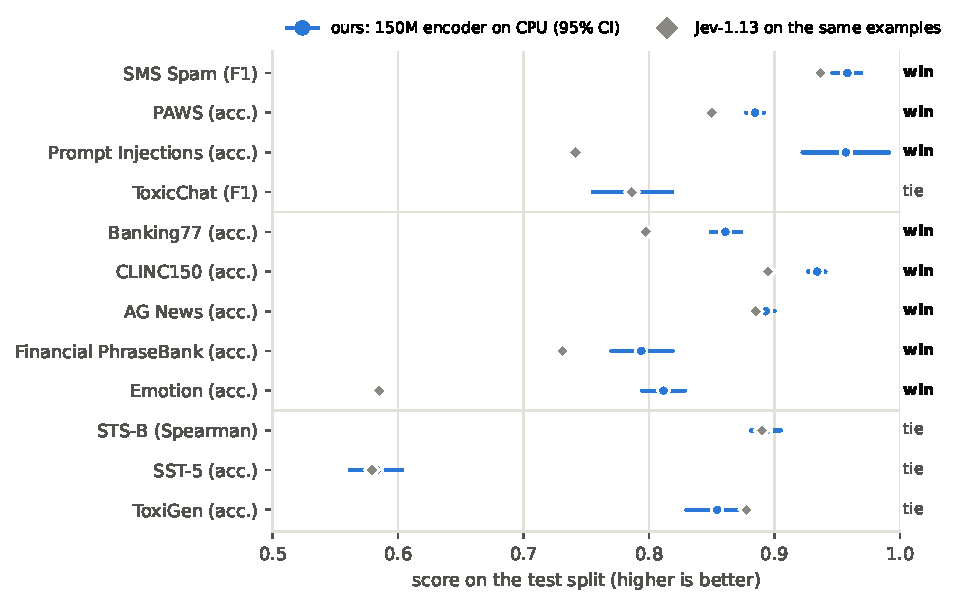
\includegraphics[width=\linewidth]{figures/results.pdf}
\caption{Test-set scores with 95\% bootstrap CIs (ours) and Jev on the same examples. Horizontal rules separate the Noul, Choice and Score tasks.}
\label{fig:results}
\end{figure}

\paragraph{Accuracy.}
Table~\ref{tab:main} and Figure~\ref{fig:results} show the results.
The owned models beat Jev on 8 of 12 tasks, with the 95\% CI entirely above Jev.
\begin{itemize}
  \item \textbf{Large margins} where Jev's zero-shot reading of the question misses the dataset's labeling convention: Emotion +0.227 and Prompt Injections +0.216.
  \item \textbf{Clear margins} on routing and domain sentiment: Banking77 +0.063, Financial PhraseBank +0.063, CLINC150 +0.039 and PAWS +0.035.
  \item \textbf{Narrow but clean wins} on SMS Spam (+0.021) and AG News (+0.008).
\end{itemize}
Four tasks are ties:
\begin{itemize}
  \item STS-B, SST-5 and ToxicChat (toxic head) are within 0.004 of Jev.
  \item On ToxicChat, the second question asked in the same request (jailbreak) is a clear win, 0.848 vs.\ 0.717.
  \item On ToxiGen our point estimate is 0.023 below Jev, with a CI that just reaches it.
\end{itemize}
In no task is our CI entirely below Jev.

\paragraph{Cost and latency.}
Table~\ref{tab:cost} and Figure~\ref{fig:cost} show the cost and latency results.
\begin{itemize}
  \item \textbf{Cost per decision:} Jev costs \$13--\$61 per million decisions, depending on prompt length. A 150M int8 encoder on four CPU threads costs \$0.52--\$1.34 at \$0.04 per vCPU-hour, which is 12--84$\times$ cheaper.
  \item \textbf{Build cost:} including every exploratory and failed experiment, it ranged from \$0.15 to \$2.57 per task (\$12.53 for all 12). It is recovered after 4k--181k decisions.
  \item \textbf{Latency:} median latency is 12--30\,ms and p95 is 19--68\,ms, below Jev's published floor. Jev's figure includes network time and ours does not; that is part of the argument for owning the model.
\end{itemize}

\begin{figure}[t]
\centering
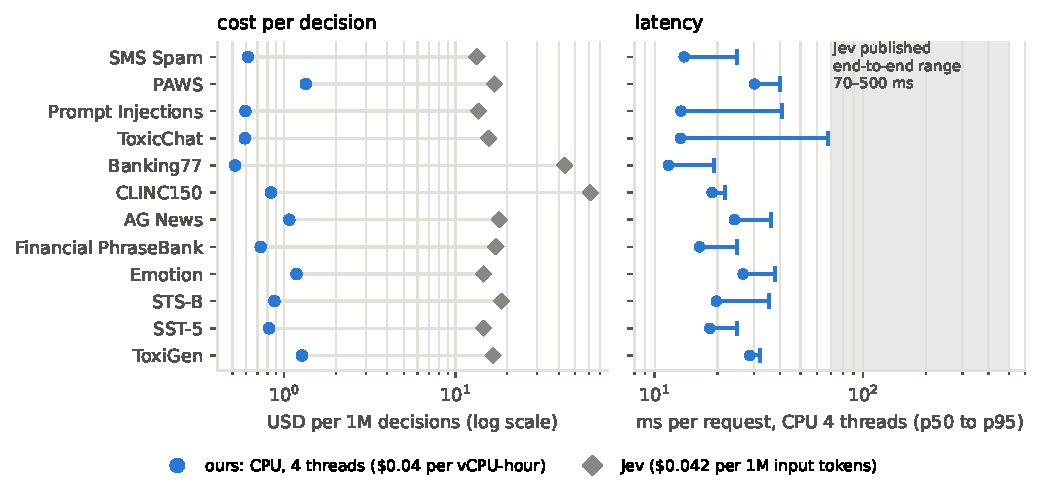
\includegraphics[width=\linewidth]{figures/cost_latency.pdf}
\caption{Left: cost per million decisions (log scale). Right: our CPU latency (dot = p50, bar end = p95) against Jev's published 70--500\,ms end-to-end range.}
\label{fig:cost}
\end{figure}
\begin{table}[t]
\centering\small
\setlength{\tabcolsep}{4pt}
\begin{tabular}{lrrrrrrr}
\toprule
 & \multicolumn{2}{c}{CPU ms} & Build & \multicolumn{2}{c}{USD / 1M dec.} & & Break- \\
\cmidrule(lr){2-3}\cmidrule(lr){5-6}
Task & p50 & p95 & cost & Jev & Ours & Ratio & even \\
\midrule
SMS Spam & 14 & 25 & \$0.23 & \$13.34 & \$0.62 & 22$\times$ & 18k \\
PAWS & 30 & 40 & \$0.31 & \$16.92 & \$1.34 & 13$\times$ & 20k \\
Prompt Injections & 13 & 41 & \$0.19 & \$13.62 & \$0.59 & 23$\times$ & 14k \\
ToxicChat & 13 & 68 & \$2.27 & \$15.64 & \$0.59 & 26$\times$ & 151k \\
Banking77 & 12 & 19 & \$0.92 & \$43.33 & \$0.52 & 84$\times$ & 21k \\
CLINC150 & 19 & 22 & \$0.24 & \$61.24 & \$0.84 & 73$\times$ & 4k \\
AG News & 24 & 36 & \$0.26 & \$18.03 & \$1.07 & 17$\times$ & 15k \\
Financial PhraseBank & 16 & 25 & \$0.15 & \$17.21 & \$0.73 & 24$\times$ & 9k \\
Emotion & 27 & 38 & \$0.38 & \$14.58 & \$1.18 & 12$\times$ & 28k \\
STS-B & 20 & 35 & \$2.57 & \$18.53 & \$0.88 & 21$\times$ & 146k \\
SST-5 & 18 & 25 & \$2.49 & \$14.58 & \$0.82 & 18$\times$ & 181k \\
ToxiGen & 29 & 32 & \$2.53 & \$16.59 & \$1.27 & 13$\times$ & 165k \\
\bottomrule
\end{tabular}
\caption{Latency and cost. CPU latency is per request (all of a task's questions), batch 1, 4 threads, worst of repeated runs on an idle Intel i9-10900X; Jev's published end-to-end latency is 70--500\,ms. \emph{Build cost} is the total OpenRouter spend for the task including every exploratory and failed experiment, so it is an upper bound on what a practitioner would pay. Jev cost uses its measured input tokens on these examples at \$0.042 per 1M input tokens; ours assumes \$0.04 per vCPU-hour. \emph{Break-even} is the number of decisions after which owning the model is cheaper.}
\label{tab:cost}
\end{table}


\paragraph{Calibration.}\label{sec:calibration}
Jev's selling point is calibrated probabilities, so a replacement must return probabilities that can be trusted, not just correct decisions.
We ran a separate post-hoc calibration study on the frozen models.
\begin{itemize}
  \item \textbf{Fitting.} For each head, the deployed model predicted the 200 gold dev examples out of sample. Where a model had trained on dev or seeds (cross-fitted SMS Spam, Prompt Injections), we used out-of-fold predictions. Candidate calibrators are none, temperature \citep{guo2017calibration}, Platt scaling and isotonic regression, chosen by 5-fold cross-validated NLL on dev and refitted on all of dev.
  \item \textbf{Decisions never change.} Choice and Score heads may only use argmax-preserving calibrators (none or temperature). Noul decisions stay at the frozen threshold on the raw probability. Accuracy and every verdict in Table~\ref{tab:main} are therefore unaffected.
  \item \textbf{One look.} Each calibrator was frozen before a single audited, logged test scoring.
  \item \textbf{Oracle rows.} As a like-for-like upper bound, we also recalibrated each system by 5-fold CV on the test labels with the same allowed methods. No deployable system could do this; it measures how much of each system's miscalibration is fixable.
\end{itemize}
Table~\ref{tab:cal} and Figure~\ref{fig:cal} show the results.
\begin{itemize}
  \item With a calibrator fitted on just 200 dev examples, our expected calibration error is lower than Jev's on 12 of 14 heads (median 0.027 vs.\ 0.086). NLL is lower on 12 of 14 and Brier score on 10 of 14.
  \item Jev is badly overconfident on Emotion (ECE 0.279, NLL 2.83), Prompt Injections (0.169) and SST-5 (0.170). On 7 of 14 heads our dev-calibrated model beats even the test-oracle recalibration of Jev in ECE, and on 9 of 14 in Brier and NLL.
  \item Jev stays better calibrated on three heads: ToxiGen's toxic head (ECE 0.014 vs.\ 0.032; Jev also has the higher AUROC there), ToxicChat's toxic head (Brier and NLL only; our ECE is lower), and CLINC150.
  \item On CLINC150 our out-of-scope rule sets the out-of-scope probability just above the best in-scope class. On the 18\% of inputs where it fires, the reported top probability is therefore about 0.28 although these predictions are mostly correct. The 200 dev examples contain only 8 out-of-scope cases, so dev selection could not detect this and kept the raw probabilities. Emitting a proper out-of-scope probability would fix it, but would change the deployed output and is left for future work.
  \item Our raw probabilities err in both directions. They are overconfident on Emotion, AG News, SST-5 and STS-B (fitted $T$ of 1.2--1.6) and underconfident on Banking77 and both ToxicChat heads ($T$ of 0.4--0.85). In every case a single parameter fitted on 200 dev examples removes most of the error.
\end{itemize}
Two rules were fixed during the study and applied to all tasks. First, the argmax-preserving restriction: two tasks had initially selected vector scaling, which can change the top choice. AG News was re-frozen before scoring. STS-B was re-scored once under a logged reason; its vector-scaling result is kept in the repository. ToxiGen's toxicity head had been scored with vector scaling, and its compliant dev choice, \emph{none}, is the raw row, so no re-score was needed. Second, the oracle rows were recomputed centrally with the same restriction, because the first version could re-classify. Both changes are recorded in the test-access log.
\begin{table*}[t]
\centering\small
\setlength{\tabcolsep}{4pt}
\begin{tabular}{llrrrrrrrrr}
\toprule
 & & \multicolumn{3}{c}{ECE} & \multicolumn{2}{c}{Brier} & \multicolumn{2}{c}{NLL} & \multicolumn{2}{c}{ECE, oracle} \\
\cmidrule(lr){3-5}\cmidrule(lr){6-7}\cmidrule(lr){8-9}\cmidrule(lr){10-11}
Task (head) & calibrator & ours raw & ours & Jev & ours & Jev & ours & Jev & ours & Jev \\
\midrule
SMS Spam & -- & 0.006 & \textbf{0.006} & 0.031 & \textbf{0.009} & 0.015 & \textbf{0.039} & 0.072 & 0.002 & 0.002 \\
PAWS & Platt & 0.051 & \textbf{0.015} & 0.020 & \textbf{0.082} & 0.109 & \textbf{0.269} & 0.348 & 0.006 & 0.005 \\
Prompt Injections & Platt & 0.023 & \textbf{0.022} & 0.169 & \textbf{0.026} & 0.192 & \textbf{0.098} & 0.590 & 0.041 & 0.067 \\
ToxicChat (toxic) & temp. & 0.061 & \textbf{0.004} & 0.015 & 0.022 & \textbf{0.020} & 0.081 & \textbf{0.074} & 0.003 & 0.006 \\
ToxicChat (jailbreak) & temp. & 0.079 & \textbf{0.005} & 0.031 & \textbf{0.005} & 0.012 & \textbf{0.023} & 0.062 & 0.001 & 0.001 \\
\midrule
Banking77 & temp. & 0.043 & \textbf{0.027} & 0.086 & \textbf{0.206} & 0.309 & \textbf{0.548} & 1.234 & 0.027 & 0.051 \\
CLINC150 & -- & 0.120 & 0.120 & \textbf{0.024} & 0.189 & \textbf{0.163} & \textbf{0.487} & 0.516 & 0.113 & 0.044 \\
AG News & temp. & 0.060 & \textbf{0.012} & 0.077 & \textbf{0.165} & 0.191 & \textbf{0.336} & 0.782 & 0.012 & 0.016 \\
Financial PhraseBank & -- & 0.054 & \textbf{0.054} & 0.137 & \textbf{0.274} & 0.383 & \textbf{0.457} & 0.703 & 0.035 & 0.017 \\
Emotion & temp. & 0.103 & \textbf{0.026} & 0.279 & \textbf{0.295} & 0.672 & \textbf{0.636} & 2.831 & 0.026 & 0.042 \\
\midrule
STS-B & temp. & 0.054 & \textbf{0.034} & 0.136 & \textbf{0.570} & 0.637 & \textbf{1.029} & 1.352 & 0.032 & 0.043 \\
SST-5 & temp. & 0.114 & \textbf{0.034} & 0.170 & \textbf{0.549} & 0.591 & \textbf{0.965} & 1.375 & 0.034 & 0.057 \\
ToxiGen (toxic) & Platt & 0.034 & 0.032 & \textbf{0.014} & 0.110 & \textbf{0.087} & 0.359 & \textbf{0.292} & 0.020 & 0.022 \\
ToxiGen (toxicity) & -- & 0.120 & \textbf{0.120} & 0.200 & 0.680 & \textbf{0.664} & \textbf{1.316} & 1.592 & 0.084 & 0.050 \\
\bottomrule
\end{tabular}
\caption{Calibration on the test split, our served model (batch size 1) against Jev on the same examples. The calibrator is chosen and fitted on the 200 gold dev examples only (5-fold CV negative log-likelihood) and frozen before a single logged test scoring; Choice and Score heads may only use argmax-preserving calibrators, so no decision changes. Score heads are scored as a distribution over levels (gold rounded to the nearest level). Bold is the better of the two systems. Ours is better on 12/14 heads in ECE, 10/14 in Brier score and 12/14 in NLL. \emph{Oracle} columns recalibrate each system by 5-fold cross-validation on the test labels with the same allowed methods: what any post-hoc recalibration of either system could reach at best.}
\label{tab:cal}
\end{table*}


\begin{figure*}[t]
\centering
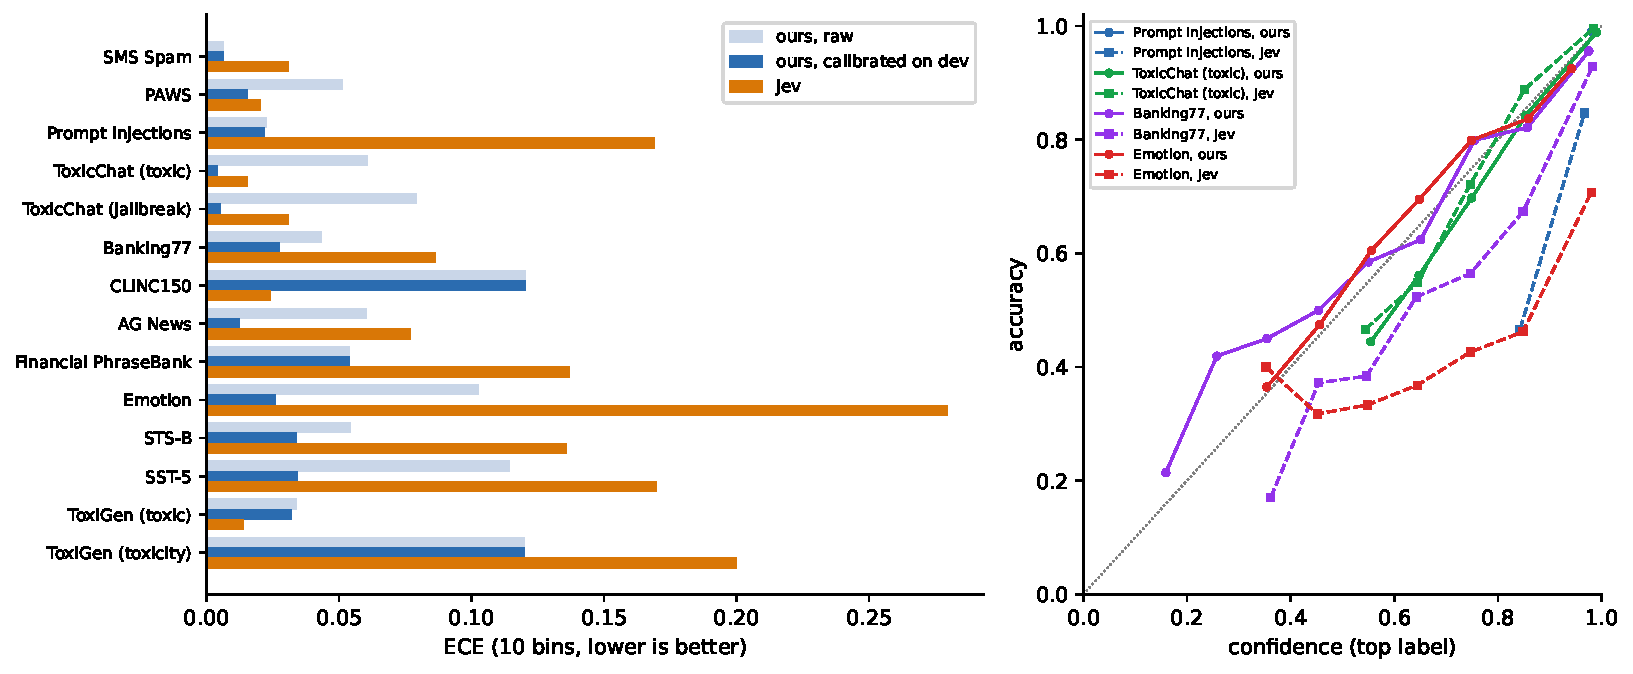
\includegraphics[width=\linewidth]{figures/calibration.pdf}
\caption{Left: expected calibration error on the test split, our served model before and after a calibrator fitted on 200 dev examples, against Jev on the same examples. Right: reliability diagrams (bins with $\geq$10 examples) for four heads; the dotted diagonal is perfect calibration.}
\label{fig:cal}
\end{figure*}

\paragraph{Serving consistency at batch size 1.}
During the calibration study, re-running the int8 models on dev did not always reproduce their frozen test probabilities.
The cause is dynamic int8 quantization: it computes activation scales over the whole input tensor, padding included, so a text's probabilities depend on the other texts in its batch.
Eight int8 tasks had computed their frozen test predictions in batches, while the model is served, and its latency measured, one request at a time.
We recomputed those predictions at batch size 1 with the same artifacts and scored them once through a separate audited script (Table~\ref{tab:batch1}).
\begin{itemize}
  \item Every verdict is unchanged. The headline metric moves by $-0.003$ to $+0.024$, and the batch-1 outputs are deterministic.
  \item Decision flips are rare on most tasks (0.3--1.5\%) but reach 3.7\% on Banking77, 5.1\% on SST-5 and 9.5\% on Financial PhraseBank. There, int8 decisions near the neutral/positive boundary are fragile, and the gain at batch 1 (0.794 to 0.818 on test) is not matched on dev (0.850 to 0.830), so it should be read as noise.
  \item Table~\ref{tab:main} keeps the pre-registered batched numbers. The calibration results above use the batch-1 predictions, with calibrators refitted on batch-1 dev predictions.
  \item ToxicChat and STS-B were already predicted at batch size 1. Emotion and ToxiGen run in fp32, where batching only adds floating-point noise.
\end{itemize}
\begin{table}[t]
\centering\small
\setlength{\tabcolsep}{4pt}
\begin{tabular}{lrlrlrr}
\toprule
Task & Batched & Batch 1 [95\% CI] & Jev & Verdict & Flips & max $|\Delta p|$ \\
\midrule
SMS Spam & 0.958 & \textbf{0.957} {\scriptsize[0.946, 0.968]} & 0.937 & win & 0.3\% & 0.41 \\
PAWS & 0.884 & \textbf{0.881} {\scriptsize[0.874, 0.888]} & 0.850 & win & 1.3\% & 0.63 \\
Prompt Injections & 0.957 & \textbf{0.966} {\scriptsize[0.931, 0.991]} & 0.741 & win & 0.9\% & 0.20 \\
Banking77 & 0.861 & \textbf{0.871} {\scriptsize[0.859, 0.883]} & 0.797 & win & 3.7\% & 0.76 \\
CLINC150 & 0.934 & \textbf{0.934} {\scriptsize[0.927, 0.941]} & 0.895 & win & 0.3\% & 0.28 \\
AG News & 0.893 & \textbf{0.893} {\scriptsize[0.886, 0.900]} & 0.885 & win & 1.5\% & 0.54 \\
Financial PhraseBank & 0.794 & \textbf{0.818} {\scriptsize[0.792, 0.842]} & 0.731 & win & 9.5\% & 0.72 \\
SST-5 & 0.583 & 0.580 {\scriptsize[0.559, 0.600]} & 0.579 & tie & 5.1\% & 0.25 \\
\bottomrule
\end{tabular}
\caption{Serving consistency of the int8 models. Dynamic int8 quantization computes activation scales over the whole input batch, so a text's probabilities depend on its batch-mates. The test predictions of these tasks had been computed in batches; here they are recomputed one request at a time, the way the model is served and its latency measured, with the same artifact. \emph{Flips}: share of test decisions that change. Every verdict is unchanged. ToxicChat and STS-B were already predicted at batch size 1; Emotion and ToxiGen run in fp32.}
\label{tab:batch1}
\end{table}

The practical lesson is to evaluate a dynamically quantized model the way it will be served, or to use static quantization when outputs must not depend on the batch.

\paragraph{Robustness to duplication.}
Some datasets repeat inputs across their own splits, and a model trained on the pool may have seen a test input's text (never its gold label).
Table~\ref{tab:dedup} re-scores the frozen predictions with exact duplicates removed.
\begin{itemize}
  \item All eight wins hold, with similar margins.
  \item ToxicChat (6\% duplicates) and ToxiGen (19\%) lean towards Jev on the de-duplicated subsets.
\end{itemize}
Those two ties should be read as ``at best on par''.
\begin{table}[t]
\centering\small
\begin{tabular}{lrrrr}
\toprule
Task & Dup.\ removed & Ours & Jev & $\Delta$ \\
\midrule
SMS Spam & 82/5354 & 0.957 & 0.936 & +0.022 \\
PAWS & 0/8000 & 0.884 & 0.850 & +0.035 \\
Prompt Injections & 0/116 & 0.957 & 0.741 & +0.216 \\
ToxicChat & 307/5083 & 0.775 & 0.790 & -0.015 \\
Banking77 & 25/3076 & 0.860 & 0.796 & +0.064 \\
CLINC150 & 19/5500 & 0.934 & 0.895 & +0.039 \\
AG News & 15/7600 & 0.893 & 0.885 & +0.008 \\
Financial PhraseBank & 4/970 & 0.795 & 0.732 & +0.063 \\
Emotion & 11/2000 & 0.814 & 0.587 & +0.228 \\
STS-B & 7/1379 & 0.893 & 0.890 & +0.003 \\
SST-5 & 2/2210 & 0.583 & 0.579 & +0.004 \\
ToxiGen & 177/940 & 0.845 & 0.879 & -0.034 \\
\bottomrule
\end{tabular}
\caption{Robustness to train/test duplication. Frozen predictions re-scored after removing test inputs that exactly match (after normalisation) any seed, dev, or training-pool text the experiment could see; Jev re-scored on the same subset. All eight wins hold; the ToxicChat and ToxiGen ties lean towards Jev.}
\label{tab:dedup}
\end{table}


\section{What mattered and what did not}\label{sec:ablations}
The 318 ledger entries let us separate the levers that moved the dev metric from those that did not.
All numbers in this section are dev numbers (200 examples) unless stated otherwise.

\paragraph{The labeling prompt was the largest lever.}
Figure~\ref{fig:labeling} shows labeler agreement with gold before and after the v2 prompt.
Guidelines written from 20 seeds and the labeler's dev errors raised agreement by:
\begin{itemize}
  \item 30 points on Emotion (0.49 $\to$ 0.785). The guideline encodes the dataset's convention that the label is the emotion word attached to ``feel'', regardless of negation.
  \item 10 points on Banking77 (0.735 $\to$ 0.84). The guideline adds descriptions for 77 intents that the question template leaves blank.
  \item 9 points on SST-5. Without guidance the labeler almost never chose ``very positive''.
  \item 6--8 points on ToxicChat, Prompt Injections, CLINC150 and STS-B.
\end{itemize}
On the half of dev never used to write the guidelines the gains are smaller but persist (Emotion: 0.60 with seeds only $\to$ 0.73 with guidelines).
Writing guidelines from errors on dev can also overfit: a second SST-5 guideline gained 4 points on the half it was written from and lost 5 on the other.

\begin{figure}[t]
\centering
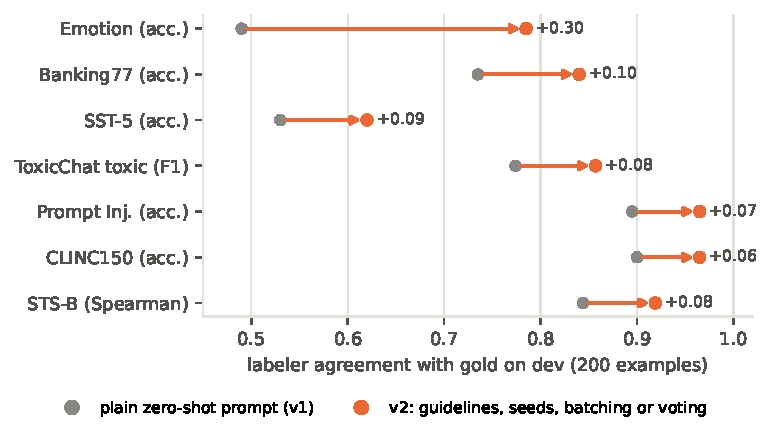
\includegraphics[width=0.85\linewidth]{figures/labeling.pdf}
\caption{Labeler agreement with gold on dev before (plain zero-shot prompt) and after the v2 prompt (guidelines from seeds and dev errors, with few-shot seeds, batching, or labeler voting depending on the task). Numbers are taken from the experiment ledgers.}
\label{fig:labeling}
\end{figure}

\paragraph{Stronger labelers rarely helped.}
For SST-5 we probed nine labelers, from \$0.03-per-million-token models up to frontier models, on the held-out dev half.
\begin{itemize}
  \item All agreed with gold at 0.52--0.60, against 0.57 for the cheap labeler.
  \item A 5-labeler average reached 0.62, with a paired CI that included zero.
  \item Enabling reasoning did not help.
\end{itemize}
On Banking77, four larger models matched but did not beat a cheap labeler with good guidelines. On ToxicChat, a frontier labeler ranked prompts best (AP 0.883) but did not improve F1.

\paragraph{Better labels do not always make a better student.}
On ToxiGen, a 4-labeler ensemble raised labeler Spearman from 0.754 to 0.818, but the student moved only from 0.770 to 0.776.
Students tend to plateau at or slightly below their labels, which makes the labeler's agreement with gold a cheap early predictor of the attainable score.

\paragraph{Data: the whole pool, and synthetic data only for gaps.}
\begin{itemize}
  \item \textbf{CLINC150:} labeling all 15k utterances instead of the exploratory round's 4.5k was the main change behind its test accuracy rising from 0.846 to 0.934. LLM-written out-of-scope utterances raised out-of-scope recall on dev from 0.81 to 0.935 at no cost to in-scope accuracy.
  \item \textbf{STS-B:} re-pairing pool sentences with their nearest neighbors, spread across the similarity scale and scored by the labeler ensemble, raised the seed-mean dev Spearman from 0.897 to 0.909. LLM-written pairs skewed to high similarity and did not help.
  \item \textbf{PAWS:} two teachers pseudo-labeled the 41k unlabeled pool pairs, and a student trained on the soft pseudo-labels reached 0.890 on dev.
\end{itemize}

\paragraph{Bigger models did not help within the latency gate.}
With the user's approval we relaxed the gate to 8 threads and allowed $\sim$400M backbones.
\begin{itemize}
  \item ModernBERT-large \citep{warner2024modernbert} matched but did not beat the 150M student on ToxiGen, SST-5 and STS-B.
  \item It exceeded 70\,ms on all but the shortest inputs.
  \item Eight threads gave only a $\sim$1.3$\times$ speed-up for a single model.
\end{itemize}
No task was re-scored under the relaxed setting.

\paragraph{Training and serving details that mattered.}
\begin{itemize}
  \item \textbf{Weight soups:} averaging fine-tunes that share an initialization worked, while averaging independently seeded runs scored below its members (STS-B).
  \item \textbf{Single-run selection:} on 200-example dev sets, seed variance often exceeded the effects being measured (four STS-B seeds of one recipe spanned 0.895--0.908), so best-of-seeds selection is optimistic.
  \item \textbf{int8 export:} plain int8 collapsed UltraBERT (accuracy 0.82 $\to$ 0.64). Keeping the MLP output projections in fp32, or using SmoothQuant rescaling, removed the loss.
\end{itemize}

\section{A recipe for practitioners}\label{sec:recipe}
\begin{enumerate}
  \item Write the question exactly as you would for Jev. Hand-label about 220 examples: 20 seeds and 200 dev.
  \item With a cheap LLM, label the seeds-plus-dev set; read the errors; write guidelines; re-check on the half of dev you did not read. Stop when agreement stops rising. This number predicts your ceiling.
  \item Label your whole unlabeled pool in batches (roughly \$0.10--\$0.30 per 10k texts with a flash-class model). Average two cheap labelers if they disagree often.
  \item Add synthetic data only for gaps such as rare classes, out-of-scope inputs, or under-covered similarity levels.
  \item Fine-tune a 150M encoder. Average 3 shared-init seeds. Fit the decision threshold on held-out data.
  \item Calibrate on the 200 dev examples with \texttt{ownyourjev calibrate}: temperature for Choice and Score heads; temperature, Platt or isotonic for Noul heads, chosen by cross-validated log-loss.
  \item Export to ONNX int8, keeping the MLP output projections in fp32. Measure CPU p95 on your hardware, and evaluate at the batch size you will serve.
\end{enumerate}

\section{Limitations}\label{sec:limitations}
\begin{itemize}
  \item \textbf{Scope.} We report the 12 classification and similarity tasks. Reading comprehension and judging generated text are future work.
  \item \textbf{Ties are not wins.} Four tasks are statistical ties. On ToxicChat and ToxiGen, duplication between the pool and test favors our models.
  \item \textbf{Test looks.} Two tasks were scored twice under the dev-gated policy. For STS-B the dev gain held on test (+0.015 on dev vs.\ +0.014 on test). For ToxicChat the second look was a latency fix that left accuracy unchanged. On tasks outside this paper, dev-gated gains shrank substantially on test, so small dev sets remain a real risk.
  \item \textbf{Human labels.} We use 220 human labels per task, while Jev is zero-shot. This is the intended comparison, since a practitioner can label 220 examples in an afternoon, but it is not label-free.
  \item \textbf{Version and latency.} We compare with \texttt{jev-1.13.0} (the published responses), and Jev's reported latency includes the network. Our latency is hardware-specific, and the cost figures depend on stated price assumptions.
  \item \textbf{Quantization.} Dynamic int8 outputs depend on the batch. We re-scored all int8 tasks at batch size 1 (no verdict changed), but on Financial PhraseBank 9.5\% of decisions are sensitive to it, so quantization-aware training would make these models more robust.
  \item \textbf{Calibration.} Calibrators are fitted on 200 dev examples, too few to see rare regions such as CLINC150's out-of-scope class. Jev remains better calibrated on three heads.
  \item \textbf{Label bias.} LLM labels inherit LLM biases. We measured agreement with gold but did not audit subgroup behavior.
  \item \textbf{AI-run experiments.} Experiments were run by coding agents under a fixed protocol. Spend caps, test access and every experiment are logged in the released ledgers. An exploratory precursor round that violated the protocol was discarded.
\end{itemize}

\section{Conclusion}
For the decisions most teams actually need, such as routing, topic, domain sentiment, spam, prompt injection, paraphrase and similarity, you do not need a hosted decision model.
A cheap LLM, an afternoon spent labeling 220 examples, and a 150M encoder on a CPU match or beat Jev on all 12 tasks we report.
The owned model's probabilities are better calibrated on 12 of 14 heads. It answers faster than Jev's best case, costs 12--84$\times$ less per decision, and recovers its build cost within thousands to a few hundred thousand decisions.
It runs where your data already is and changes only when you retrain it.
The code, the per-task ledgers and the audited test log are available at \url{https://github.com/erfaneshrati/ownyourjev}.

\bibliographystyle{plainnat}
\bibliography{refs}

\appendix
\section{Per-task recipes}\label{app:recipes}
All students are fine-tuned end-to-end. ``Soft'' denotes training on per-option probabilities.
\begin{itemize}
  \item \textbf{SMS Spam:} gte-modernbert-base, 5-fold cross-fit; deepseek-flash labels with seed examples; int8.
  \item \textbf{PAWS:} UltraBERT-150M; flash labels with seeds plus soft pseudo-labels on 41k unlabeled pairs from two UltraBERT teachers; partial int8 (attention matmuls and \texttt{down\_proj} kept in fp32).
  \item \textbf{Prompt Injections:} gte-modernbert-base; 326 pool texts labeled with seed-derived guidelines (labeler dev accuracy 0.965), 1,148 seed-steered synthetic EN/DE inputs, and the 220 gold examples; int8.
  \item \textbf{ToxicChat:} one gte-modernbert encoder with two heads; soft labels averaged from two cheap labelers, plus synthetic hard positives and negatives; uniform soup of 7 shared-init runs; eager-attention export with SmoothQuant; thresholds from dev.
  \item \textbf{Banking77:} gte-modernbert; soft vote labels from four labelers (two on the whole pool, two adjudicating 840 disagreements), using a prompt with hand-written intent descriptions and all 220 gold examples; int8.
  \item \textbf{CLINC150:} gte-modernbert; the whole 15k pool labeled in batches of 20 with intent descriptions; 2,066 synthetic out-of-scope utterances; out-of-scope threshold 0.4; int8 on the MLP input projections only.
  \item \textbf{AG News:} gte-modernbert; 5k flash labels; int8.
  \item \textbf{Financial PhraseBank:} gte-modernbert; 3.6k flash labels with seeds; int8.
  \item \textbf{Emotion:} gte-modernbert; 10k flash labels with the ``feel-word'' guideline and seeds; fp32 ONNX (int8 cost 2 dev points).
  \item \textbf{STS-B:} gte-modernbert; 4-labeler averaged soft scores with SemEval guidance, sentence-swap augmentation, 7.6k re-paired pool pairs, and a 3-run shared-init soup; int8 with the MLP output projections kept in fp32.
  \item \textbf{SST-5:} UltraBERT-150M; soft labels with SST-convention guidance and seeds; partial int8.
  \item \textbf{ToxiGen:} one gte-modernbert encoder with two heads; soft labels for $P(\text{toxic})$ and a 5-level distribution; \emph{toxic} derived as expected level $/4 \ge 0.30$ (chosen by CV on dev); fp32 ONNX.
\end{itemize}

\section{Test-access log}\label{app:log}
Table~\ref{tab:log} lists every test scoring of the 12 reported tasks. Both re-scorings carry logged evidence:
\begin{itemize}
  \item STS-B: 7.6k re-paired pairs plus a shared-init soup; dev $+0.015$, CI $[+0.004, +0.028]$.
  \item ToxicChat: an idle-machine re-measurement showed the first model exceeded the latency gate (p95 68--75\,ms). The fix (eager export plus SmoothQuant) left dev F1 unchanged.
\end{itemize}
The full log, including the deferred tasks, is in \url{benchmarks/results_v2/TEST_ACCESS.log}.
\begin{table}[h]
\centering\small
\begin{tabular}{llrrl}
\toprule
Time & Task & Ours & Jev & Kind \\
\midrule
2026-10-18 19:52 & SMS Spam & 0.9580 & 0.9366 & first scoring \\
2026-10-18 20:00 & Financial PhraseBank & 0.7938 & 0.7309 & first scoring \\
2026-10-18 20:14 & AG News & 0.8930 & 0.8850 & first scoring \\
2026-10-18 20:16 & Banking77 & 0.8609 & 0.7975 & first scoring \\
2026-10-18 20:49 & CLINC150 & 0.9340 & 0.8949 & first scoring \\
2026-10-18 21:47 & STS-B & 0.8791 & 0.8900 & first scoring \\
2026-10-18 22:04 & ToxiGen & 0.8543 & 0.8777 & first scoring \\
2026-10-18 22:16 & Emotion & 0.8115 & 0.5850 & first scoring \\
2026-10-18 22:31 & SST-5 & 0.5828 & 0.5792 & first scoring \\
2026-10-18 23:53 & PAWS & 0.8845 & 0.8499 & first scoring \\
2026-10-18 23:55 & Prompt Injections & 0.9569 & 0.7414 & first scoring \\
2026-10-19 01:11 & ToxicChat & 0.7875 & 0.7862 & first scoring \\
2026-10-19 01:31 & STS-B & 0.8935 & 0.8900 & re-score (dev-gated) \\
2026-10-19 02:59 & ToxicChat & 0.7870 & 0.7862 & re-score (latency gate) \\
\bottomrule
\end{tabular}
\caption{Every test scoring of the 12 reported tasks, from the audited log. The log also records 23 analysis-only accesses (calibration, batch-1 serving, oracle recompute, de-duplication) (Section~\ref{sec:calibration}), none of which changed a model, a threshold or a decision.}
\label{tab:log}
\end{table}


\end{document}
